\documentclass[twoside,11pt,openright]{report}

\usepackage[latin1]{inputenc}
\usepackage[american]{babel}
\usepackage{a4}
\usepackage{latexsym}
\usepackage{amssymb}
\usepackage{amsmath}
\usepackage{epsfig}
\usepackage[T1]{fontenc}
\usepackage{lmodern}
\usepackage[labeled]{multibib}
\usepackage{color}
\usepackage{datetime}
\usepackage{epstopdf}
\usepackage{graphicx}
\usepackage{subcaption}
\usepackage{hyperref}
\usepackage{enumitem} %Used to make lists smaller

\renewcommand*\ttdefault{txtt}

\newcommand{\todo}[1]{{\color[rgb]{.5,0,0}\textbf{$\blacktriangleright$#1$\blacktriangleleft$}}}

% \newcites{A,B}{Primary Bibliography,Secondary Bibliography}

% see http://imf.au.dk/system/latex/bog/

\begin{document}

%%%%%%%%%%%%%%%%%%%%%%%%%%%%%%%%%%%%%%%%%%%%%%%%%%%%%%%%%%%%%%%%%%%%%%%

\pagestyle{empty} 
\pagenumbering{roman} 
\vspace*{\fill}\noindent{\rule{\linewidth}{1mm}\\[4ex]
{\Huge\sf An Artificial Neural Network Approach: Combining Green Energy Production and Electricity Price Forecasts to Support Green Decision Making}\\[2ex]
{\huge\sf Brian Bak Laursen, 20071275}\\[2ex]
{\huge\sf Kristan Barret, 20073457}\\[2ex]
\noindent\rule{\linewidth}{1mm}\\[4ex]
\noindent{\Large\sf Master's Thesis, Department of Computer Science, ICT Product Development\\[1ex] 
\monthname\ \the\year  \\[1ex] Advisor: Niels Olof Bouvin\\[15ex]}\\[\fill]}

\epsfig{file=logo.eps}\clearpage

%%%%%%%%%%%%%%%%%%%%%%%%%%%%%%%%%%%%%%%%%%%%%%%%%%%%%%%%%%%%%%%%%%%%%%%

\pagestyle{plain}
\chapter*{Abstract}
\addcontentsline{toc}{chapter}{Abstract}

\todo{in English\dots}

\chapter*{Resum\'e}
\addcontentsline{toc}{chapter}{Resum\'e}

\todo{in Danish\dots}

\chapter*{Acknowledgements}
\addcontentsline{toc}{chapter}{Acknowledgments}

\todo{\dots}

\vspace{2ex}
\begin{flushright}
  \emph{Brian Bak Laursen,}\\
  \emph{Aarhus, \today.}
\end{flushright}

\tableofcontents
\pagenumbering{arabic}
\setcounter{secnumdepth}{2}

%%%%%%%%%%%%%%%%%%%%%%%%%%%%%%%%%%%%%%%%%%%%%%%%%%%%%%%%%%%%%%%%%%%%%%%

\chapter{Introduction}
\label{ch:intro}
\section{The Problem}
Renewable energy has become increasingly important. Energy suppliers make it possible for their customers to choose between green and brown energy. Companies and persons promote themselves with green profiles to get a certain kind of image and it has become a choice of the individual company or home to be green. This is only one part of the picture, because the increased attention on green energy is influencing the market forces behind the scenes where acquisition of energy begins \cite{windPowerDanishLiberalized}. Various trading companies buy electricity on the deregulated energy market and since the amount of renewable energy in this market is increasing and will do for the years to come\cite{6, windPowerDanishLiberalized} the traders need to consider it carefully when buying and selling. The most essential task and basis for any decision making in the power market is to forecast the electricity price \cite{pjmForecast} and wind power production \cite{dayAheadImpactOfWindPowerForecasts}. Traditional producers can use the wind power predictions to strategically place their own energy in the market \cite{21}.
\\[0.5cm]
The electricity market consists of two instruments in order to facilitate trading between producers and consumers of energy: the pool which works as an online marketplace, and a framework to make physical contracts possible between both parties \cite{21}. The producers can make their electricity available and the consumers can bid correspondingly. An auction is made every hour to decide the market clearing price and which bids are accepted for that hour. The consumers and producers need to predict the hourly clearing prices to make plans for which bidding strategies to use. If a trader has a precise day-ahead prediction of the prices it will be easier to maximize profit by using the best possible strategy for exactly those conditions \cite{21}. The electricity traders will attempt to buy electricity in a low-price market and sell it when the price has come up like in other commodity markets \cite{FIND REF}. With a precise prediction they know when to buy and when to sell. 

Approximately 25\% of the total power production in Western Denmark was covered by wind power in 2008 and influenced the prices on the power market accordingly \cite{windPowerDanishLiberalized}. The impact on price is seen in wind power variations in areas where wind power production covers a substantial amount of the total supply which apply for Denmark. For this reason it cannot be avoided when predicting electricity prices\cite{dayAheadImpactOfWindPowerForecasts}. Since the amount of green energy in the entire Danish liberalized market is targeted to increase to 30\% by 2025 which is almost a doubling since 2008 \cite{windPowerDanishLiberalized} the influence will only become greater. The price impact from windmills will be even greater in strong wind periods and in areas with congestions in the power transmission capacity \cite{windPowerDanishLiberalized}. The increase in renewable energy makes the ability of predicting green energy production and the corresponding market price more vital. It is not trivial to predict wind production because green energy by nature is unpredictable, e.g. wind power is highly influenced by wind speed and air density. If the traders are able to predict wind power when doing actual price forecasts it will give rise to a huge advantage in the market when deciding to buy or sell \cite{dayAheadImpactOfWindPowerForecasts}. Price forecasting itself contains many other factors than wind power that needs to be considered equally \cite{21}.
\\[0.5cm] Traders buy and sell in real-time, intra-day or day-ahead \cite{FIND REF}. This puts constraints on a price prediction algorithm --- but what constraints depend solely on the type of trade. If the trader wishes to buy in real-time or hour-ahead the algorithm must perform and deliver a result within minutes or seconds. If it is day-ahead then the time-interval can be increased. This might result in a compromise on the margin of error because fast results make less time for analysis and computation. Another fact is that the closer you get to the time of the trade the more accurate the weather predictions will be which directly impacts the price prediction algorithm using it. The ability to make both short- and long-term forecasts is very important in the deregulated competitive electricity market because it helps the trader to reduce risks in terms of under/over estimating the revenues from potential sales and this of course also makes it easier to manage risk\cite{21}.
\\[0.5cm]
Demand has a huge influence on the electricity price. No demand, no electricity price, but if these were the only two variables to consider, a linear regression model could be used for establishing a relationship and thereby a prediction. Other dynamic elements have an impact on the price and therefore the linear regression approach would result in the presence of serial correlation in the error \cite{21}. For instance will overestimated energy prices for one year most likely lead to overestimates the next year since it does not account for all the dynamic parameters. It is necessary to carefully consider all variables and characteristics of the price that we are trying to predict in the electricity market and then use a model that handles correlated errors based on this. The most noticeable characteristics are \cite{21}:
\begin{itemize}
\item High frequency;
\item High volatility;
\item Unusual prices in times of very high demand;
\item Calendar effect (weekend, holidays);
\item Multiple seasonality (daily and weekly periodicity);
\end{itemize}
When doing electricity price forecasting these characteristics must be taken into consideration when modelling a prediction algorithm. 

\todo{describe how green decision making is important due to the regulation of prices if the consumption can be covered by the amount of green energy. This makes it important to identify the green energy.}

\subsection{Price Prediction Systems}
The stock price movements have similarities with electricity prices in terms of its non-linearity and chaotic/dynamic nature. Investors must take into account these factors when handling time series that are non-stationary, noisy and have structural breaks\cite{stockForecasting}. In addition, macro-economical elements significantly influence stock and electricity prices, e.g the economy in general, politics, bank rates and expectations of investors could be examples of such influences. In \cite{stockForecasting} they presented an Artificial Neural Network (ANN) approach to forecasting stock prices. These networks are powerful tools when solving complex problems because they possess qualities such as learning, generalizing, parallel processing and error endurance. The ANN in \cite{stockForecasting} is based on a Wavelet De-Noising-based Back Propagation (WDBP) that has the ability to filter away undesirable characteristics from the input. The purpose of the filtering is to separate stock price characteristics away from noise so that the prediction will have better chances of accuracy when all undesirable noise has been discarded. The prediction is then used by investors in their attempt to gain profits. 

A day-ahead forecasting algorithm that predicts electricity prices in the market based on Artificial Neural Network (ANN) and Similar Days Method (SDM) is described in \cite{pjmForecast}. The purpose is to give close estimates for several days to come. The estimates can be used by electricity traders in their decision making but also by transmission companies for different purposes. The companies can use it for scheduling a short-term generator outage in order to predict where it is most inexpensive. It can also be used by actual producers of energy to strategically bid into the market to increase prices. The price estimate itself plays a big role in decision making in all of these examples.

The combination of ANN and SDM is an attempt to simplify the ANN and make the prediction more accurate. The SDM technique averages five days that are similar to the corresponding forecast day. This makes the algorithm consider the influence of the most similar days and their price development compared to the day we wish to forecast. An actual forecast can be seen in figure ~\ref{fig:actualForecastMay13}.
\begin{figure}[!ht]
\centering
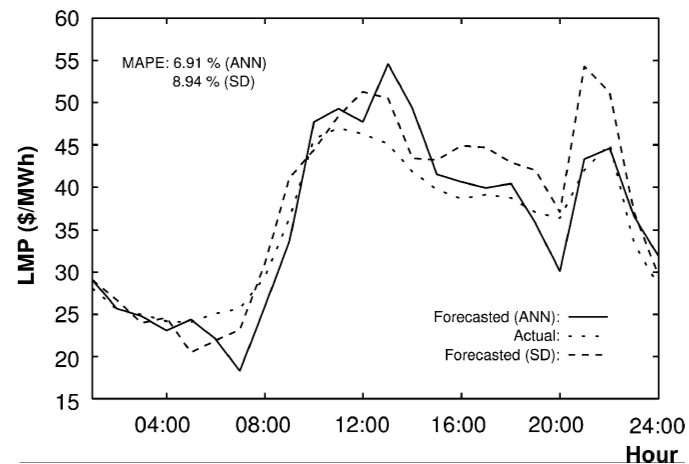
\includegraphics[width=0.8\linewidth,natwidth=898,natheight=587]{billeder/SDMANNAccuracy.png}
\caption{Actual day-ahead forecast from Saturday, May 13, 2006 \cite{pjmForecast}}
\label{fig:actualForecastMay13}
\end{figure}
The ANN is trained with 45 days from the day before the forecast, 45 days before and after the forecast day in the previous year.
\\[0.5cm]
Prediction algorithms are not only used by electricity traders but can also be a part of various applications. In \cite{22} they introduce an intelligent electricity broker (IEB) that is integrated into Smart Grids where it; 1) provides provision of en energy storage; 2) attempts to lower the electricity bill, and 3) optimally utilizes electricity during peak and low-peak energy production periods. The prediction algorithm is used by a decision algorithm to locate points in time where it is most feasible for the owner of the smart grid to either sell stored energy or buy energy if storage is low. It helps the system to lower the total amount of energy costs to the owner and also utilize the energy in the most intelligent way.
 

\subsection{Green Energy Production}
When dealing with prediction of green energy production it is necessary to look at the weather in more detail. Wind power prediction can be divided into two areas \cite{5}: 1) time-series analysis of power data and 2) wind speed prediction and conversion to power. What needs to be utilized in wind power prediction is wind speed and wind direction which of course has a big influence on how much energy a wind turbine generates. An approach to analysis and prediction of wind power generation is presented in \cite{WindPowerGenerationUsingANN} where an Artificial Neural Network is used to predict the production. The prediction is based on weather data such as wind speed, relative humidity but also for how many hours the windmill is generating power.

Another source of green energy is solar panels. Solar
prediction algorithms are very accurate when the weather conditions are steady but in changing weather a large error margin is seen. To predict power output from a solar farm the time-series prediction algorithms and Estimated Weighted Moving Average (EWMA) models can be used \cite{5}.

The prediction of wind power can be used en various contexts. Data centers is an example of a place where green energy prediction can be useful. It is often necessary for data centers to run long-running batch jobs where performance is measured in how many jobs it completes and the throughput. In \cite{5} they design an adaptive job scheduler that utilizes prediction of solar and wind energy production to scale workload. Earlier work has focused on using immediate available green energy and then cancelling and rescheduling jobs thereafter. The point in \cite{5} is instead to scale the number of jobs to the expected availability of green energy production by predicting it beforehand. This helps reducing the number of cancelled jobs as the jobs are then scheduled for whenever the energy is available. If the amount of green energy production is not sufficient for an immediate or emergency job the remainder will be covered by brown energy. The system reduces the amount of wasted green energy and increases the overall throughput of the data center.
\\[0.5cm]
In this thesis we will only be focusing on green energy that originates from windmills.


\subsection{Decision Support Systems}
Decision Support Systems (DSS) can help users in critical environments where careful situation assessment and decision making is necessary. This is valid for the financial markets such as the stock and electricity market where multiple dynamic factors are present \cite{UncertainInformation}.
\\[0.5cm]
A combination of an Artificial Neural Network approach, an eXtended Classifier System (XCS) and the idea of cooperative learning is presented in \cite{groupLearningDS}. It is an attempt to incorporate the best of all three in an intelligent financial decision support system. XCS and ANN are both forecasting technologies and the system compares their results in order to get the best price estimate. The cooperative learning element shows itself in the way a decision is made. Each agent selects the best investment strategy from their own point of view based on the price estimates. The agents can simulate several strategies in each session and select the potential of highest profit. This information is shared with the rest and the final investment decision is made based on the decision of the majority of the other agents in the system. The DSS archives investment strategies that showed to be profitable in a premium strategy library in order to collect the best strategies. The agents do not necessarily have to use the premium strategies but it makes sense to first try what have succeeded in the past and if that fails move on to a random selection strategy. 

The intelligent system described above makes all decisions for the agent as opposed to the HCI approach to DSS discussed in \cite{UncertainInformation}. The focus is on uncertain information and how to present it to the user in the best possible way. They argue that uncertain information cannot be denied and especially not in the domains with high risks such as the financial markets and military systems. The underlying reasoning algorithm used by the system will still make qualified estimates but the final decision is left to the user. The system will inform about uncertainties so the user can make trade-off's based on the information and then make a decision. Uncertainties can exist as different types such as bad data source reliability, conflict in data and data ambiguity but no matter the type it is presented to the user at all time. 

In \cite{UncertainInformation} is further discussed how to present information including linguistic, textual and graphical so that it is perceived better and faster by the user. Finally they present a number of guidelines that can used to develop a prototype of the interface for a DSS.

\section{The Method}
The available data are prices, wind productions and meteorological factors measured every hour from earlier years. When variables are observed sequentially over time it constitutes a time series where the values in the series evolve over time. Furthermore time series data are often strongly correlated over time which make it usable for prediction \cite[Chapter~7.1.2]{econometrics}. Based on the data and the non-linear nature of price forecasting and energy price prediction we want a system that is able to develop and learn from the past by analysing the time-series. Artificial Neural Networks can be categorized as Machine Learning \cite{18} and are networks that imitate the behaviour of the human brain \cite{1}. We choose to base our system on ANN because it gives us the power to be able to forecast energy prices based on how the prices have evolved in the past. Our decision is based on the nature of Artificial Neural Networks and how it is used in machine learning. It is often used in non-linear statistical analysis \cite{16} and has been used to predict various prices within the commodity market \cite{2,3,stockForecasting,pjmForecast}. We have chosen to use a multi-layered feed forward architecture since this is one of the most used and widely implemented in open-source frameworks \cite{17}.

We will base our work on Artificial Neural Networks and the Resilient Backpropagation (RPROP) algorithm used to train the network in order to predict electricity prices and wind power generation. The RPROP algorithm is a learning algorithm that uses weights to analyze the input dataset\cite{17} and it is a faster algorithm than its predecessor Backpropagation \cite{8,15}. It is commonly used on the feedforward architecture and is the most used and implemented algorithm on ANNs \cite{14,17}.
<<<<<<< .mineWe will base our work on Artificial Neural Networks and the resilient backpropagation (RPROP) algorithm used to train the network in order to predict electricity prices and wind power generation. It is faster than its predecessor Backpropagation \cite{8,15}.  The RPROP algorithm is a learning algorithm that uses weights to analyze the input dataset and to configure further learning \cite{17}. It is commonly used on the feedforward architecture and is the most used and implemented algorithm on ANNs \cite{14,17}. The historical data to include in the dataset will be identified through a systematic analysis of the electricity price and wind power characteristics together with experiments for verification. The result will be the optimal network settings for prediction of wind power and electricity prices in relation to best network structure, input, representation, size of training set and number of training epochs. The findings of our analysis and experimental results will be related to practical use in terms of decision making.=======We will base our work on Artificial Neural Networks and the Resilient Backpropagation (RPROP) algorithm used to train the network in order to predict electricity prices and wind power generation. The RPROP algorithm is a learning algorithm that uses weights to analyze the input dataset\cite{17} and it is a faster algorithm than its predecessor Backpropagation \cite{8,15}. It is commonly used on the feedforward architecture and is the most used and implemented algorithm on ANNs \cite{14,17}.

The prediction algorithm will be based on historical data which potentially could be a very large dataset. The more historical data included in the algorithm the more data needs to be processed. We need to analyse how much of this data is necessary for precise prediction and perhaps make tradeoffs to ensure performance for decision support.>>>>>>> .theirs

\section{The Hypothesis}
In this dissertation we take our outset in the growing need for green decision making. It is our intent to forecast green energy production and electricity prices within the electricity market by modelling an Artificial Neural Network using the back propagation algorithm for training of the network. The dataset for training consists of historical data that is relevant to the specific task. For instance when dealing with forecasting of wind power production for a wind farm, the most influential factors are meteorological such as wind speed, wind direction and air density together with historical production development of that particular farm. The energy prices are also influenced heavily by meteorological factors but it is instead combined with historical price development.
The goal is to investigate whether or not Back Propagation Artificial Neural Networks are a proper technology for doing prediction of green energy and electricity prices. Secondly, we are discussing the actual use of Artificial Neural Networks as Decision Support.
\\[0.5cm]
We will be focusing on; 1) modelling and implementing a working Back Propagation Artificial Neural Networks that are capable of predicting price and energy production within the electricity market; 2) evaluating predictions originating from Artificial Neural Networks in terms of both results and actual decision making.


%%%%%%%%%%%%%%%%%%%%%%%%%%%%%%%%%%%%%%%%%%%%%%%%%%%%%%%%%%%%%%%%%%%%%%%

\chapter{Main Concepts}
This chapter will introduce and explain the technologies and concepts that are the foundation for the thesis.
\label{ch:foundations}
\section{Machine Learning}
Machine learning algorithms can figure out how to perform tasks by generalizing, where the goal is to generalize beyond the examples of a training set \cite{18}. The programs using the algorithm learn from data and as more data becomes available, more complex problems can be handled. Systems such as web search, spam filters and stock trading uses this approach.
\\[0.5cm]
Many learning algorithms exist and they are all based on combinations of three components \cite{18}; 1) the \textbf{representation} component makes an attempt to discover how to represent the input during training of the algorithm. What kind of information expressed in the data decides what representation algorithm to use; 2) the \textbf{evaluation} component has the objective of distinguishing between the best and the worst output from the representation component and let the next component decide which choice is the best. Basically it attempts to map the output to a specific value so that the next component can analyze it; 3) finally, the \textbf{optimization} component needs to search for the highest scoring output from the evaluation and then deliver it as a result. A greedy search could be an example of such a search (see figure ~\ref{fig:threeComponents}).
\begin{figure}[h!]
\centering
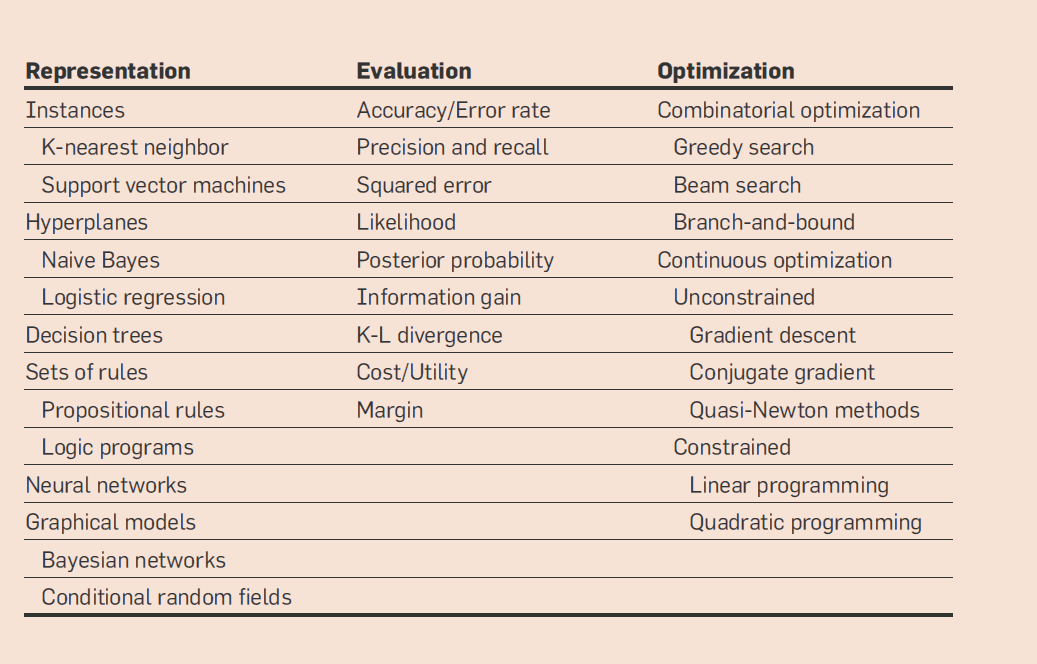
\includegraphics[width=0.6\linewidth,natwidth=898,natheight=587]{billeder/Table1-TheComponentsOfLearningAlgorithms.png}
\caption{The three components of learning algorithms \cite{18}}
\label{fig:threeComponents}
\end{figure}
\\[0.5cm] 
Machine learning cannot rely on data alone. Every learner must make assumptions beyond the data that is given to generalize beyond it \cite{18} because it is not possible to map the real world uniformly to a possible mathematical function. When meteorologists try to model the weather they make assumptions based on historical datasets that are similar to the current weather conditions. If enough historical occurrences resulted in the same weather condition the meteorologists must make the assumption that it can be classified as what have been seen before. The same is applicable when predicting electricity prices. We examine historical data and locate situations that are similar to the current and if enough examples with the same result is found it can be assumed that they are of the same type.
\\[0.5cm]
It can be the case that the system is not at all able to deliver a correct answer. This could result in the system guessing to the best of its ability or simply randoming an answer. This problem is called overfitting \cite{18}. Overfitting can be divided into bias and variance, where bias is when the learner consistently learns the same wrong thing over and over again. Variance is the learner's tendency to learn random things and ignoring the possibility of a more correct answer. See figure ~\ref{fig:biasandvariance} for an example with dart throwing.
\begin{figure}[h!]
\centering
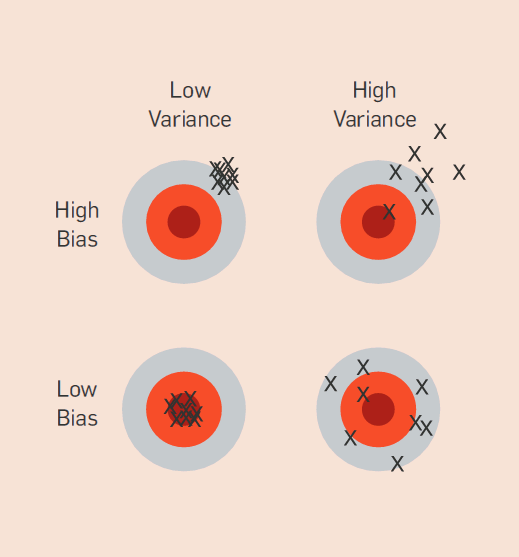
\includegraphics[width=0.5\linewidth,natwidth=898,natheight=587]{billeder/biasVSvariance.png}
\caption{Example of bias and variance in a dart throw \cite{18}}
\label{fig:biasandvariance}
\end{figure}

Machine learning is not only about the technical stuff but it also relies a great deal on intuition, creativity and  black art \cite{18}. 
\newline A way to achieve machine learning is by using a Artificial Neural Network. One way to model an ANN is to base it on the
Levenberg-Marquardt algorithm \cite{7,9,10}. It is a least squares algorithm that,
opposed to Backpropagation algorithm\cite{8}, is very fast at calculating the
results. It is a curve fitting algorithm mostly used on nonlinear problems with
a lot of unknowns[Need citation]. The algorithm can be used with Artificial Neural Networks and information approximation\cite{8} and it can be used in combination with the backpropagation algorithm to be used on a feedforward architecture of the neural network\cite{13}.

%%%%%%%%%%%%%%%%%%%%%%%%%%%%%%%%%%%%%%%%%%%%%%%%%%%%%%%%%%%%%%%%%%%%%%%
\newpage
\section{Artificial Neural Network}

This section is based on information from the book AI techniques for game programming\cite{buckland2002ai} chapter 7, 8 \& 9. Also from the book Neural networks: a systematic introduction\cite{rojas1996neural} chapter 7.
\\[0.5cm]
Neural networks are models that imitate the brains behavior. They have been created as an option to model artificial intelligence and analyze machine learning. The human brain is made up of billions of neurons that are interconnected in a big grid. They communicate by firing electrical shocks through the network of neurons. The human brain is extremely complex and can calculate vast amounts of data in no time. This is why scientists and mathematicians have been trying to emulate this behavior to create artificial intelligence.

\begin{figure}[!ht]
\centering
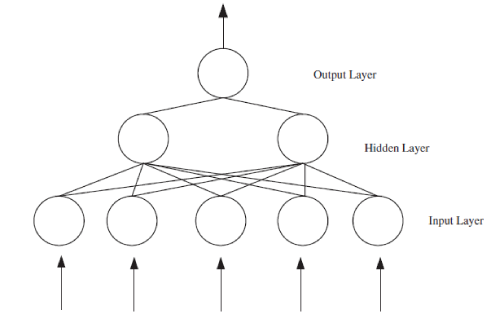
\includegraphics[width=0.8\linewidth,natwidth=898,natheight=587]{billeder/ANN.png}
\caption{A simple neural network with 3 layers. \cite{stockForecasting}}
\label{fig:ANN}
\end{figure}

Artificial neural networks (ANN) are artificial neurons (nodes) that are connected in a network. The network consists of an arbitrary number of layers that are interconnected. The most common structure in these networks are a feed forward structure. This kind of structure has the characteristic that it only flows data from the input layer through the layers to the output layer. There are no loops in the network thus making it unable to reiterate any information. Normally all of the nodes in the input layer is connected to all of the nodes in the second layer. The same connections are done in the next layers until we hit the output layer. This will give us the sum of all the previous nodes($x_i$) and their weights($w_i$)($\sum_{i=0}^{i=n+1} w_i x_i$) in every node in the next layer. See ~\ref{fig:weight_of_layers}.
\begin{figure}[!ht]
\centering
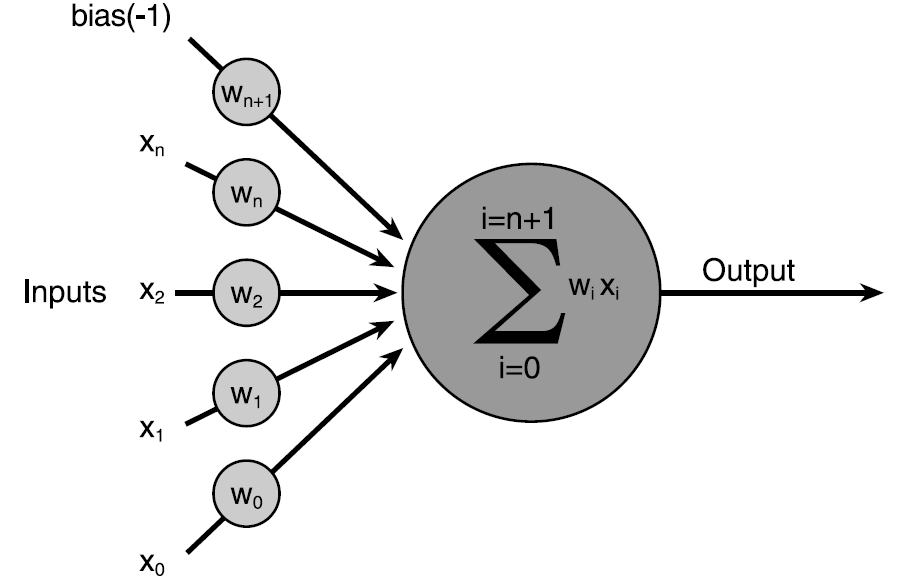
\includegraphics[width=0.8\linewidth,natwidth=898,natheight=587]{billeder/weight_of_layers.png}
\caption{How the weight is calculated from one layer to the next}
\label{fig:weight_of_layers}
\end{figure}
All of these connections carry a weight that dictates how data flows through the network and reflects the relations between the inputs and the outputs of the network. The inputs of the network should be all the factors that has an influence on the output we want from the network. In our example we would want to input; weather data, temperature, demand, availability \cite{21} to get the price as an output from the network.

Every node in our network contains an activation function. This function, when calculated, tells us whether the artificial neuron should fire or not. That is, if the neuron should transmit the data from the current layer to the next layer. There are a lot of different activation functions. The simplest form is the binary step function which either fires or it does not. This depends on the input and gives us a low threshold of complexity which is good in simple neural networks as the relations between the nodes do not need to be that fine grained. In more complex systems we want activation functions with a broader output range than binary. In many cases a sigmoid function is used as the activation function. This is because of the ''S''-shape which enables it to compute outputs in a non-linear way. The non-linear nature of the sigmoid functions is what makes the neural network able to compute non-trivial problems in reasonable sized networks. The sigmoid function allows the activation functions of the neurons to have a broader range of inputs which will produce an output compared to step activation functions. To be able to calculate a non-trivial problem in these kind of networks we need what is called a training algorithm. This algorithm depicts how the network evolves over time also known as learning. There are two kinds of learning; supervised learning and unsupervised learning.

\subsection{Unsupervised learning}
Unsupervised learning is when we do not have prior data to base our work on. Instead we have a problem where we want the neural network to try and estimate its behaviour relative to a specific task based on some assumptions we have about the system it performs on. It is commonly used with estimation problems like "Cluster Analysis", which in short is attempting to fit data into clusters of data that have some of the same criteria. This is often done by exploring the dataset and that is what unsupervised learning is good for. It also works with Artificial Intelligence(AI) that have to explore parts of the (virtual)world. In \cite{buckland2002ai} he explains how an unsupervised learning feed-forward artificial neural network trains itself using a genetic algorithm to keep track of the fitness function of the AI. The fitness function is used to tell the AI if it is doing good or doing bad and is used to train the network. It will get a plus score in the fitness function if it encounters what we are looking for and get negative if it hits something that we defined as "wrong". Based on this fitness function it will update the weights of the neural network accordingly to what is most beneficial for the network as a total. After it has been allowed to do a lot of runs it begins to get a sense of what it is exploring and should be able to make better choices for each run.

\subsection{Supervised learning}
Supervised learning are a set of algorithms that use a dataset which contains both the inputs and from those inputs what the output is expected to be. This dataset is used to train the neural network to make it able to do calculations on current data and predict the outcome. An example of an algorithm used for supervised learning is the back-propagation algorithm. 
It starts out by randomly assigning weights to all of the connections between the neurons. It then calculates the output of the network and compares it to the expected output. From that it calculates the error margin between the expected and the calculated output and adjusts the weights accordingly. This is done for all the hidden layers (as well) until we hit the input layer. All of these steps are called an epoch. We will repeat as many epochs as we need until the sum of all the errors are within a given threshold. The name of the algorithm originated from this approach where it propagates the error backwards in the network.

Supervised learning can be thought of as learning with a teacher. As an example we can use the XOR table:

\begin{table}[!ht]
\centering  % used for centering table
\begin{tabular}{c c c} % centered columns (3 columns)
Input \#1 & Input \#2 & Output \\ [0.5ex] % inserts table 
%heading
\hline                  % inserts single horizontal line
0 & 0 & 0  \\ % inserting body of the table
1 & 0 & 1  \\
0 & 1 & 1  \\
1 & 1 & 0 \\ [1ex] % [1ex] adds vertical space
\hline %inserts single line
\end{tabular}
\caption{This training set is very simple yet it illustrates a training set for a supervised learning algorithm very well.} % title of Table
\label{table:xor-table} % is used to refer this table in the text
\end{table}

In this dataset we have both of the inputs and we are given the expected output. This gives the back-propagation algorithm a direction to follow when minimizing the error function of the network. We can do this because we get an output that we can compare to the expected output which allows us to predict the direction that the error correction should take to come closer to the answer. Also the sigmoid activation function helps us closing in on the target output since the sigmoid function always has a positive derivative which ensures that we will always have a direction to follow\cite[p. 153]{rojas1996neural}. This is because the derivative of the sigmoid function always will point us towards the global minima of the expected function. If we take a look at ~\ref{table:xor-table} we are given inputs and outputs. We take the input 1 and 0 and we expect the output to be 1. The neural network will initialize weights and start to run the back-propagation. The back-propagation algorithm will compare the output it gets to the output we expected e.g. we may get an output of 0.5 (based on the random weight initialization) and this is compared to the expected output 1. Because of the sigmoid function we know what direction the weights should be corrected to come closer to the output of 1. This allows the back-propagation algorithm to recalculate the weights and be sure that it is heading for the global minima of the error function thus heading for the right output.
%[FORKLAR MATEMATIKKEN EVT MED EKSEMPEL s. 332 i bogen]

In neural networks bias neurons are often added to the layers to help them learn patterns. The bias neurons are added to give the activation functions the ability to change its output even if x is zero. If we look at the graph in figure ~\ref{fig:activationFunctions} it uses the following activation function: \begin{math} \frac{1}{(1+e^{(-cx)})} \end{math} where c is the weight.

\begin{figure}[!ht]
\centering
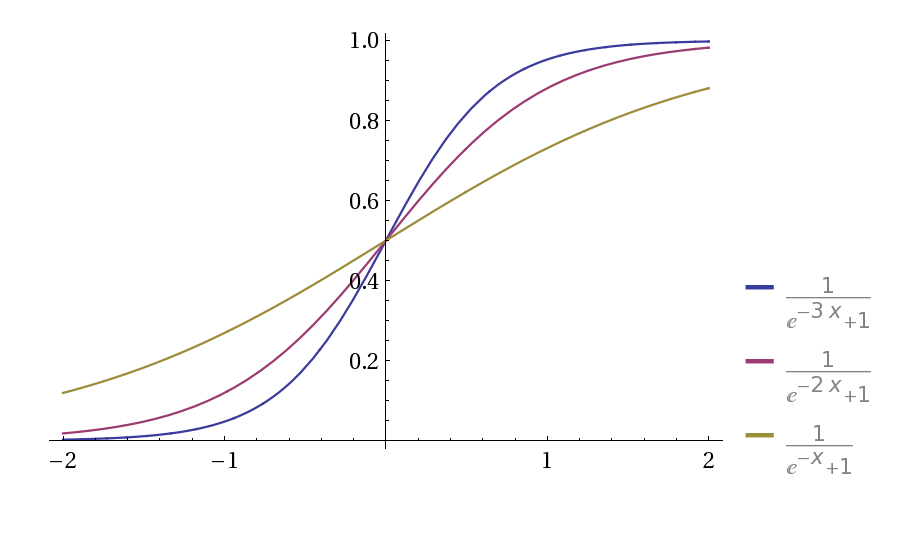
\includegraphics[width=0.8\textwidth ,natwidth=410,natheight=237]{billeder/ActivationFunctions.png}
\caption{}
\label{fig:activationFunctions}
\end{figure}

The figure shows how the gradient of the function alters with different weight values. Even though the gradient of the function is clearly altered by the weights the function is still outputting the same result for zero thus we cannot alter the output for x equal to zero just by altering the weights. This is what we use the bias for. If we apply a bias of one to all of the neurons we will be able to shift it either to the left or the right. In figure ~\ref{fig:activationFunctionsWithBias} we see the same function as before where the weight is set to 2. The difference is that we added a bias (b) to this function: \begin{math} \frac{1}{(1+e^{(-2x+b)})} \end{math} \cite[p. 165]{rojas1996neural} \cite{inductiveBias}

\begin{figure}[!ht]
\centering
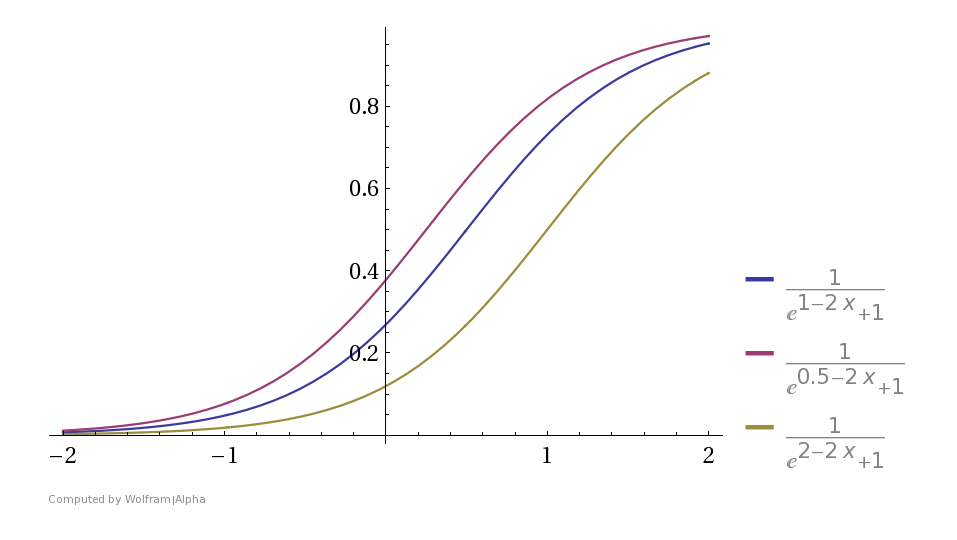
\includegraphics[width=0.8\textwidth ,natwidth=410,natheight=237]{billeder/ActivationFunctionsWithBias.png}
\caption{}
\label{fig:activationFunctionsWithBias}
\end{figure}

To calculate the error between input and output we use the mean squared error function. This function is given by: \begin{math} MSE=\frac{1}{n}\sum_{i=0}^{n}(\hat{y}_i-\bar{y}_i)^2 \end{math} where \begin{math} \hat{y}_i \end{math} is the ideal value and \begin{math} \bar{y}_i \end{math} is the actual value. We use this error calculation because it incorporates the bias \cite{meanSquaredError}

\subsection{Common pitfalls}
When we are trying to fit our algorithm and make it recognize patterns we will encounter several possible pitfalls. First of all there is the chance of ending up in a local minima. This is when the the back-propagation algorithm attempts to find the global minimum of the error curve, thus having reduce the error as much as possible. The algorithm works by trying to reduce this error margin a little step at a time. If it encounters a local minima on the curve and thinks it has reached the global minima it gets stuck and we will get inaccurate results ~\ref{fig:localMinimum}. 

\begin{figure}
\centering
\begin{minipage}{.5\textwidth}
  \centering
  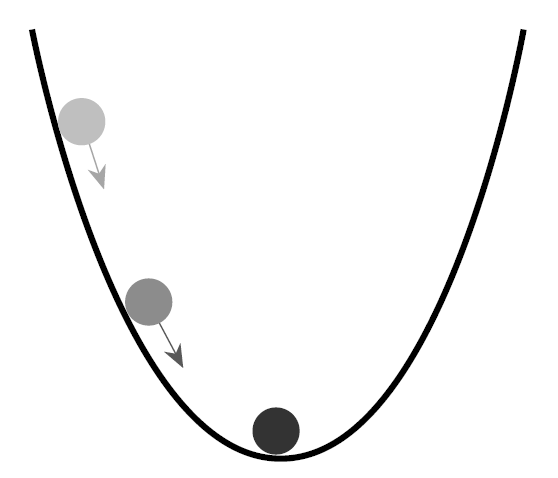
\includegraphics[width=.4\linewidth]{billeder/globalMinimum.png}
  \captionof{figure}{At the global minimum \cite[P. 318]{buckland2002ai}}
  \label{fig:globalMinimum}
\end{minipage}%
\begin{minipage}{.5\textwidth}
  \centering
  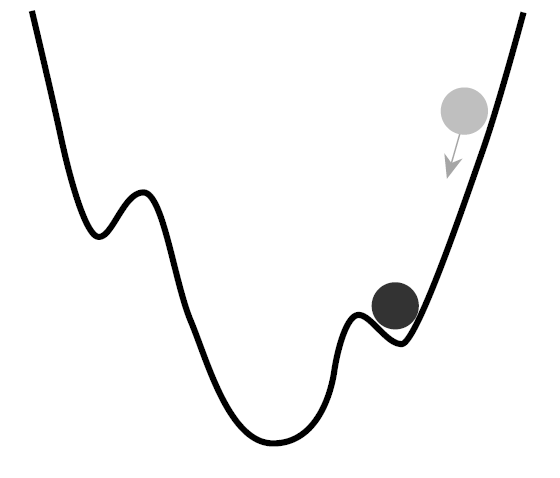
\includegraphics[width=.4\linewidth]{billeder/localMinimum.png}
  \captionof{figure}{Stuck in a local minimum \cite[P. 318]{buckland2002ai}}
  \label{fig:localMinimum}
\end{minipage}
\end{figure}

To avoid the backpropagation algorithm to falsely accept a local minima as the global minima we can give the algorithm momentum. This is done by adding a bit of the last error correction from the earlier layer to the next layers error correction. This way the algorithm, so to say, will scoot right by any small deviations in the error correction face.
\newline
Another pitfall when working with neural networks is over fitting the algorithm. This is when the algorithm instead of finding a generalized pattern in the inputs it will find an over-fit pattern that will fit exactly that input. This is better shown in figure ~\ref{fig:overfitting}.
\begin{figure}[!ht]
\centering
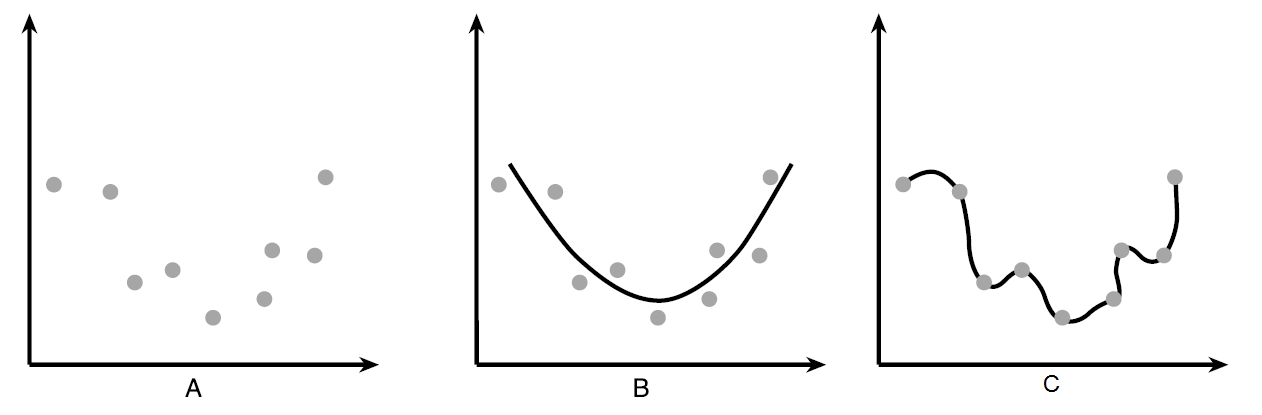
\includegraphics[width=0.8\linewidth,natwidth=1262,natheight=415]{billeder/overfitting.png}
\caption{A. The plot graph of the input B. The generalized function C. An over-fit function \cite[P. 319]{buckland2002ai}}
\label{fig:overfitting}
\end{figure}
This can be avoided by some simple techniques. First of all we want to reduce the neurons as much as possible as long as it does not interfere with our performance of the system. This is a trial and error problem and has to be tweaked along with evolving your neural network. We can add noise to avoid this problem. By adding noise(random data values) we prevent the algorithm from fitting the function to closely to the given data. Thus giving us a more generalized function where it hopefully will be able to fit new data presented to it better. Early stopping is another method to avoid over-fitting. This is only doable with large datasets where you can split it into two equal datasets. The first will work as a training set and the second will work as a validation set. We will keep training the dataset and checking with the validation set until the difference between those two start to increase.

\subsection{Summary}
This section touched the basics of neural networks and where the inspiration for these networks came from. It summed up what architecture we focus on in this paper namely the feed-forward architecture. This architecture allows data to only flow from input to output with no loops in it. We elaborated what activation functions are and how they are used in neural networks. In our neural network we are gonna use the more complex version called a sigmoid function which resembles and S if you draw it. This is done because it gives a wider variety of outputs than a normal step function. Since neural networks are all about the computer learning to calculate some very complex problem we need a learning algorithm. We explained that unsupervised learning algorithms are about exploring possibilities in a space and try to come close to a goal that we set up. It has no definitive goal (opposed to supervised learning) but a success factor that it tries to maximize. As mentioned we also talked about supervised learning and how these algorithms try to achieve the best possible result. This is done by trial-and-error where the algorithm learns until it satisfies an error margin we chose. Furthermore we talked about why and what bias is used for. It is a constant that is added to the calculations to prevent the algorithm to stall while trying to find the lowest error margin in our prediction. We also explained common pitfalls and how to avoid these. Among these were over-fitting of the function we are trying to a achieve which means it only fits the training set and not a general set of data. Also we talked about the algorithm falsely believing that the local minima was the global minima and therefore coming up with a wrong result.
We also talked about the training set and how this data is handled by the training algorithm. We mainly focus on supervised training since this is what we are gonna use in this thesis. A very important point to make here is that the training set is of utmost importance when it comes to performance and accuracy of our ANN. The training set has to be developed and refined during a training period of a network and relies a lot on experience and tinkering with the inputs. We need to normalize the input set so that it fits each other and all the parameters get the same weighting from the beginning. This is done not to favor any input unintentionally and vice versa. Also we can only have assumptions of on which form the inputs will give the best result and we might have to try different forms like numbers, bits, bitmaps etc. to get the best results. Also we might have a reason to think some data is important but that it turns out it just makes the calculations more complex without adding any nuance to the output and therefore can be omitted from the calculations.
All in all we tried to give a brief introduction to neural networks and the technologies that we use with it.

%%%%%%%%%%%%%%%%%%%%%%%%%%%%%%%%%%%%%%%%%%%%%%%%%%%%%%%%%%%%%%%%%%%%%%%
\newpage
\section{Prediction}
Being able to predict electricity prices and green energy production is the basis for our thesis. Demand has a huge impact on the electricity price so this is also handled here. This section will introduce and give selected examples of these concepts within the different areas. 

\subsection{Electricity Demand}
Weather conditions have a impact on the electricity industry in terms of network infrastructure and electricity consumption. In \cite{19} they describe a multiple regression model that accurately predicts the monthly electricity demand based on weather and sociocultural conditions. The monthly electricity demand from this model shows a clear cyclic pattern which reflects the temperature changes during the year \cite{19}. Besides from weather conditions, social and economic factors also affect the monthly demand, e.g. the demand was decreased in Denmark during the \fnurl{financial crisis in 2009}{http://www.business.dk/investor/finanskrisen-saetter-elforbrug-i-bakgear}.

\subsubsection{Parametric multiple regression}
Parametric multiple regression is preferred in \cite{19} as opposed to an Artificial Neural Network used in this thesis. From a statistical error indices point of view they describe that the Artificial Neural Network (ANN) is a valid choice for prediction. The argument for multiple regression is the simplicity in adjusting input values for each analysis of electricity demand in the prediction model. 

To make a demand prediction based on weather conditions they have established a relationship between the two. To get an understanding of this relationship they have made a plot of the average monthly demand as a function of Central England Temperature (CET) \cite{19}. The plot (see figure ~\ref{fig:CET}) shows an inverse relationship where it can be seen that a lower temperature in general results in an increased load consumption. Winter gives rise to lighting and heating load which is consistent with lower temperatures, and conversely in the summer with temperatures above 18 degrees the consumption tends to increase again due to the need for cooling and air-condition \cite{19}.
\begin{figure}[h!]
\centering
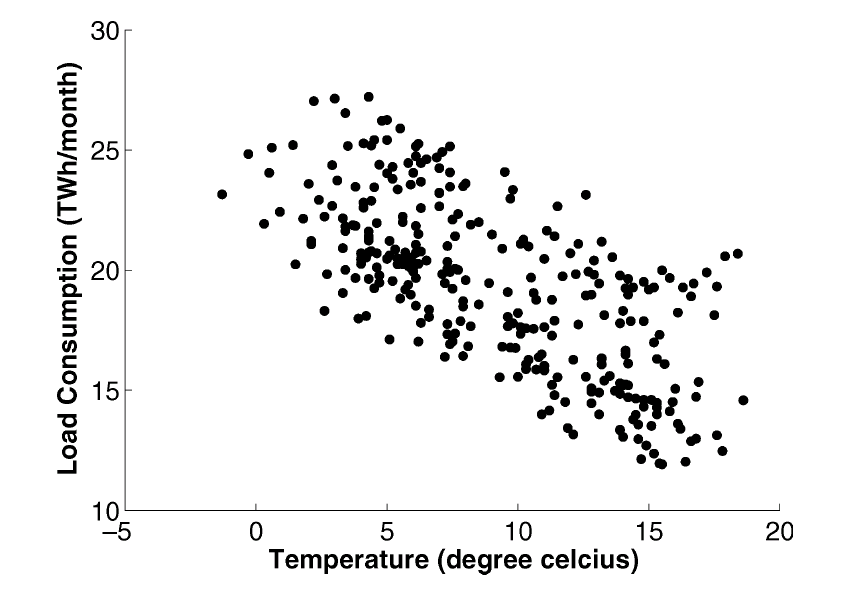
\includegraphics[width=0.8\linewidth,natwidth=898,natheight=587]{billeder/MeanMonthlyDemandEngland.png}
\caption{Function of monthly CET as a function from 1970 to 1995 \cite{19}}
\label{fig:CET}
\end{figure}

\subsubsection{Heating and Cooling Degree Days}
The nonlinear relationship between temperature and load consumption is turned into a concept called degree days. They introduce two categories of days; 1) Heating Degree Days (HDD) that is used to quantify when heating is required; 2) Cooling Degree Days (CDD) which is then used to quantify the need for cooling. The days are calculated from the CET data and give a more indicative picture than the temperature-load relationship \cite{19}. A simple explanation of the calculation follows.
\begin{center}
$CDD=\sum\limits_{d=1}^{N_{d}}(\gamma_{d})(T_{dm}-T_{base_{C}})$
\end{center} 
 
where $T_{base_{c}} = 20^{\circ}$ is the base temp and $T_{dm}$ is the mean daily temperature. $\gamma_{d} = 0$ if $T_{dm}-T_{base_{c}} < 0$ and $\gamma_{d} = 1$ if $T_{dm}-T_{base_{c}} > 0$. In other words if the temperature is above $20^{\circ}$ the day can be characterized as CDD and there is a need for cooling.
\begin{center}
$HDD=\sum\limits_{d=1}^{N_{d}}(1-\gamma_{d})(T_{base_{H}}-T_{dm})$
\end{center} 

where $T_{base_{h}} = 15.5^{\circ}$ is the base temp and again $T_{dm}$ is the mean daily temperature. $\gamma_{d} = 1$ if $T_{base_{h}}-T_{dm} < 0$ and $\gamma_{d} = 0$ if $T_{base_{h}}-T_{dm} > 0$. This means that on a day with temperatures below 15.5 degrees there is a need for heating. In both cases where $\gamma_{d} != 0$ a big difference has a greater impact on the demand.

Temperature is the most influential factor but other weather conditions can also be used when predicting the electricity demand, e.g. wind speed and rainfall can impact heating and lighting demand whereas direct sunshine can decrease the need for heating \cite{19}. The model can be expressed by the relation between all factors by adding them together, e.g. the HDD value automatically increase the total electricity demand if it is not zero and this apply to all other factors in the model seen below.

\begin{center} \^E$_{A}=\alpha_{0}+\alpha_{1}CDD+\alpha_{2}HDD+\alpha_{3}ELD
+\alpha_{4}V_{w}+\alpha_{5}M_{s}+\alpha_{6}M_{r}$ 
\end{center} 
 
Where $\alpha_{n}$ are constants, ELD is humidity, $V_{w}$ is wind speed, $M_{s}$ sunshine and $M_{r}$ rainfall.
The calculation model can also include socio-economic factors. Specifically the population growth has a natural impact on the electricity demand over time. The more people the higher the demand gets. This would give rise to an additional factor in the model considering the growth. The prediction model from \cite{19} comes within 3 percentage of the actual demand when it is run on data from 1996-2003 which they consider to be close (~\ref{fig:predicteddemand}).
\newline
\begin{figure}[h!]
\centering
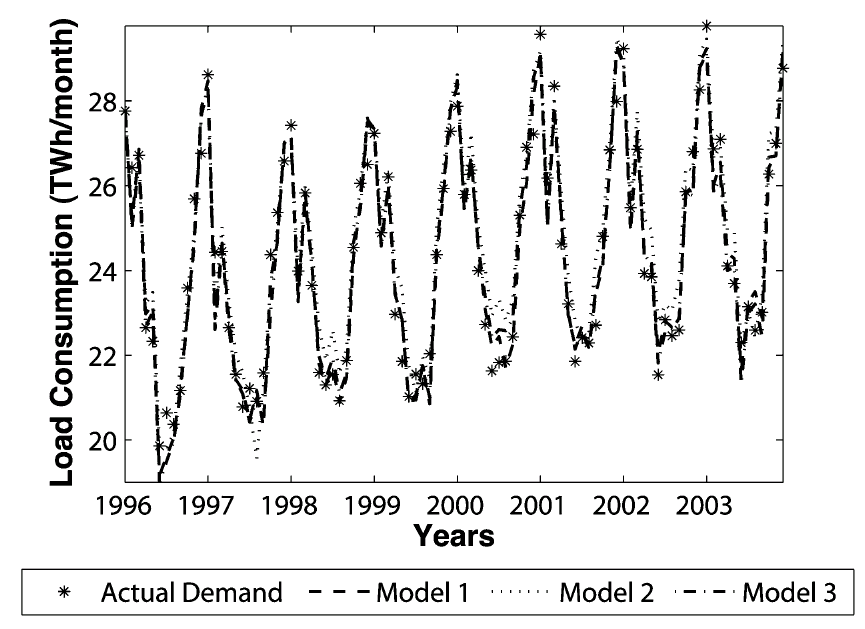
\includegraphics[width=0.8\linewidth,natwidth=898,natheight=587]{billeder/PredictionOfDemand.png}
\caption{The actual values and the predicted demand in a comparison \cite{19}}
\label{fig:predicteddemand}
\end{figure}

\subsubsection{Summary}
The electricity demand has great influence on the energy price. It is important to identify the influences of the demand because those inevitably also will have an affect on the electricity prices. 

The concept of Cooling Degree Days (CDD) and Heating Degree Days (HDD) has been described. They might give us an quantifiable parameter to measure the need for cooling and heating in Denmark. What it brings forward is the necessity for considering demand when predicting price and a potential of substituting demand with the parameters given --- wind speed, temperature, ect. The demand function (\^E$_{A}$) is presented. This function gives a picture of the factors that directly influence the demand and the possible mappings to our ANN as the demand part --- every parameter is an input.

\subsection{Wind Power Production}
The identification of rich wind resources have become important together with the increasing focus on green energy \cite{WindPowerGenerationUsingANN}. It is important to analyse and predict the wind power generation at a certain location before placing actual windmills. 
Wind speed, relative humidity and generation hours of the windmills are used as input for a Artificial Neural Network in \cite{WindPowerGenerationUsingANN}. It can come as no surprise that the meteorological factors like wind speed and air density have a huge impact on the wind power generation. Figure~\ref{fig:energyGeneration} shows how the monthly energy generation increases with the monthly average wind speed. 

\begin{figure}[h!]
\centering
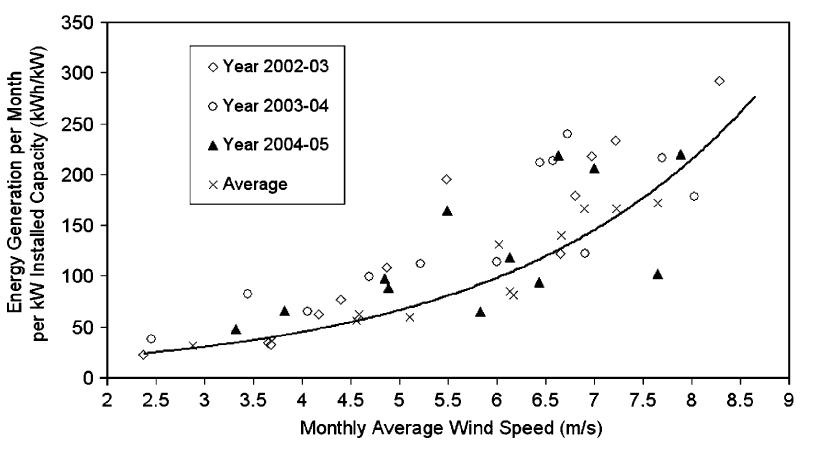
\includegraphics[width=0.8\linewidth,natwidth=898,natheight=587]{billeder/EnergyGenerationVsWindSpeed.png}
\caption{The influence of wind speed on the energy generation \cite{WindPowerGenerationUsingANN}}
\label{fig:energyGeneration}
\end{figure} 

The more "heavy" the air, the more energy is received by the windmill turbine. The humidity increases as as air density increases and because wind energy is proportional to air density the prediction algorithm needs humidity as input because it also accounts for temperature and pressure \cite{AirDensityInForecast}. Moist air is lighter than dry air because water molecules are less dense than the molecules in dry air such as oxygen and nitrogen. This basically means that the more air molecules like oxygen and nitrogen the more wind energy.

The last parameter in their prediction algorithm is generation hours which is the period in which the turbines produce power. The number of hours are influenced by f.x mechanical breakdowns, scheduled maintenance and low wind speeds. It is clear the the more generation hours the more energy is produced as seen in figure ~\ref{fig:energyGenerationFromHours}. The generation hours are hard to predict but can be calculated from past years up-time together with the expectations of the company delivering the windmills.  

\begin{figure}[h!]
\centering
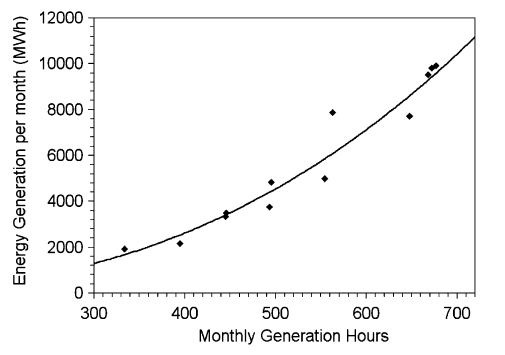
\includegraphics[width=0.8\linewidth,natwidth=898,natheight=587]{billeder/GenerationHourVSGeneration.png}
\caption{The influence of generation hours on energy production \cite{WindPowerGenerationUsingANN}}
\label{fig:energyGenerationFromHours}
\end{figure} 

The Artificial Neural Network trains 3-year dataset containing the mentioned input parameters. The input parameters are during the training compared to the output variable which is the wind energy output of the turbine. See figure~\ref{fig:annArchitecture} for the architecture.
\\[0.5cm]
\begin{figure}[h!]
\centering
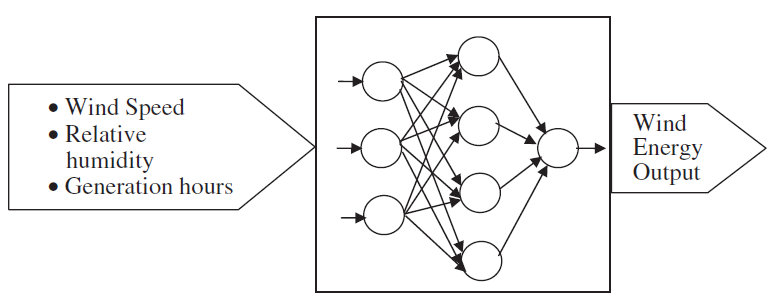
\includegraphics[width=0.7\linewidth,natwidth=898,natheight=587]{billeder/ANNwindSpeedPrediction.png}
\caption{Artificial Neural Network architecture from \cite{WindPowerGenerationUsingANN}}
\label{fig:annArchitecture}
\end{figure}

\subsection{Electricity Prices}
A day-ahead forecasting algorithm that predicts electricity prices in the market based on Neural Network (ANN) and Similar Days Method (SDM) is described in \cite{pjmForecast}. The purpose is to give close estimates for several days to come. The estimates can be used by electricity traders in their decision making but also by transmission companies for different purposes. The companies can use it for scheduling a short-term generator outage in order to predict where it is most inexpensive. It can also be used by actual producers of energy to strategically bid into the market to increase prices. The price estimate itself plays a huge role in decision making in all of these examples.

The combination of ANN and SDM is an attempt to simplify the ANN and make the prediction more accurate. The algorithm forecasts by using a ANN that modifies price curves obtained by averaging five similar price days corresponding to the forecast day, i.e. The ANN corrects the received output from the similar days approach \cite{pjmForecast}. In other words the technique takes into consideration the influence of the most similar days and their price development in relation to the day we wish to forecast.

The ANN is trained with only 45 days from the day before the forecast and 45 days before and after the forecast day in the previous year \cite{pjmForecast}. Results can be seen in table~\ref{table:sdmresult}

\begin{table}[h!]
\centering  % used for centering table
\begin{tabular}{c c c} % centered columns (3 columns)
Year 2006 \#1 & ANN (Avg. MAPE [\%]) \#2 & ANN ( FMSE [\$/MWh] ) \\ [0.5ex] % inserts table 
%heading
\hline                  % inserts single horizontal line
January 20 & 6.93 & 4.57  \\ % inserting body of the table
February 10 & 7.96 & 6.12  \\
March 05 & 7.88 & 5.39  \\
April 07 & 9.02 & 5.87 \\ [1ex] % [1ex] adds vertical space
\hline %inserts single line
\end{tabular}
\caption{Results of forecasting from \cite{pjmForecast}.} % title of Table
\label{table:sdmresult} % is used to refer this table in the text
\end{table}


An explanation for the choice of days is not discussed in the paper. As  mentioned in \cite{18} the more data the more complex problems can be handled

Artificial Neural Networks (ANN) has also been used for electricity price forecasting. In \cite{singhal2011electricity} they use an ANN to predict the half-hourly price of electricity of 24 hours. They differentiate between three different kinds of days: Normal trend price, Price with small spikes and price with large spike. They present a prediction for each of these days and present us to the mean absolute error and the root mean square error, which are standard measures for how accurately the prediction is done. The neural network is fed with 13 inputs as follows \cite{singhal2011electricity}:
\begin{itemize}[noitemsep,topsep=3pt,parsep=2pt,partopsep=3pt]
\item Day of week
\item Time slot of Day
\item Forecasted Demand
\item Change in demand
\item Price (one day ago) - 3 inputs 
\item Price (one week ago) - 3 inputs
\item Price (two weeks ago) - 1 input 
\item Price (three weeks ago) - 1 input 
\item Price (four weeks ago) - 1 input
\end{itemize}
These inputs are fed into a 4-layer neural network: one input layer, two hidden layers and an output layer. The analysis of their ANNs shows that neural networks make a very precise prediction on normal trend price days but have difficulties forecasting the price with small and large spikes. They argue that if the reasons to the spikes in the price were taken into account as inputs in the network maybe the network would be better at forecasting the spikes prices. Also they argue that fuzzy logic, neural networks and dynamic clustering together will provide more efficient forecasting of the prices.
\\[0.5cm]
Since price forecasts in electricity markets are such a volatile operation because of the shifting tides, price demand, holidays etc. that affects the price it can be a cumbersome problem to model. In \cite{amjady2006day} he proposes a new method based on neural networks and fuzzy logics to predict the electricity prices. He calls the new network approach a new fuzzy neural network. Fuzzy logic is basically a logic that has many values or many correct answers. Opposed to binary logic sets, where the answer can be only true or false, in fuzzy logic we have several grades of what we define as true, thus making it harder to decide what is really the truth but also makes us available to have a way larger scale of the data we are looking at.

The fuzzy logic is used within the nodes in the hidden layer to do evaluation of the data inputs. That is the activation function of the neurons in the hidden layer contains a fuzzification function that creates a square of the inputs compared to sinus activation functions that normally takes the sums of the inputs. This square over the inputs is used to classify the inputs into hyper cubes (input spaces) and then calculating how close they are together. Calculation of how far the inputs are from each other are used to calculate the output of the functions. By this we will get an upper and lower limit that the inputs can range between and thus we get a input that has the characteristics which turns out to give a better result than ARIMA, wavelet-ARIMA, MultiLayered ANNs and Radial Basis based ANNs. The data however is not optimized in this paper and they claim this to be future work. They also state that the better performance is based on a limited dataset.

\subsubsection{Arima Prediction}
 The Auto Regressive Integrated Moving Average (ARIMA) model is a time series model where the ARIMA processes analyse time series with a class of stochastic processes \cite{EnergyPriceForecasting,ARIMA}. The model has been applied to forecast of commodity prices such as oil, gas and electricity \cite{ARIMA}. 

The success of the presented ARIMA model is dependent on the linear relationship of the underlying data generating process, whereas the Neural Network can handle non-linear relationships \cite{1}. The Neural Networks are simple but a very powerful tool when it comes to forecasting, provided that the training set contains enough data and that enough computational resources are available. 
In \cite{1} the Neural Network outperforms the ARIMA model in terms of both time consumption and accuracy of the predicted price as shown in ~\ref{fig:ArimaVSNN}. where the error percentage to the actual price is shown.
\begin{figure}[h!]
\centering
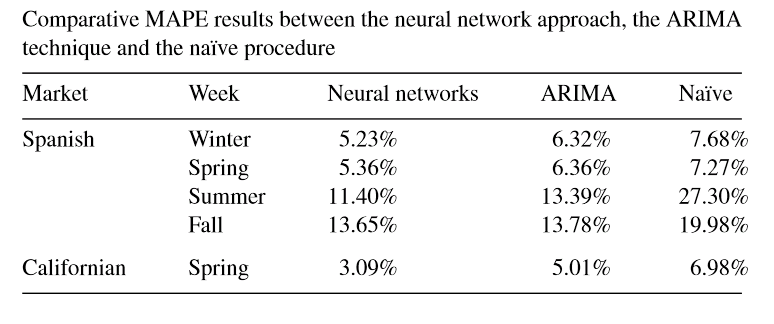
\includegraphics[width=0.8\linewidth,natwidth=898,natheight=587]{billeder/ARIMAvsNN.png}
\caption{Comparison between Neural Network and ARIMA in terms of error \cite{1}}
\label{fig:ArimaVSNN}
\end{figure}
\subsubsection{Support Vector Machine Prediction}
Support vector machines (SVM) can be used for forecasting in the commodity market. In \cite{xie2006new} they use SVMs for predicting the crude oil prices. SVMs are by nature a linear learning machine which means SVMs always use linear functions to solve the regression analysis. However they can be expanded to be able to solve nonlinear problems. This is done by mapping the data into a high-dimensional feature space using a nonlinear mapping. Afterwards it is possible to use linear regression on this space to solve nonlinear problems. The SVMs undergo four different phases before being able to make predictions. These can be seen in figure ~\ref{fig:phasesOfSVM}
\begin{figure}[weight!]
\centering
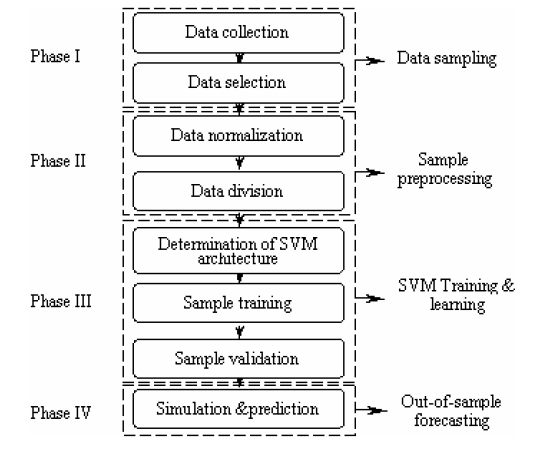
\includegraphics[width=0.8\textwidth ,natwidth=410,natheight=237]{billeder/phases_of_SVM.png}
\caption{The steps taken to create a Support Vector Machine}
\label{fig:phasesOfSVM}
\end{figure}
Data sampling is done daily but due to inconsistencies in these data they adopt weekly and monthly data as alternatives. Data preprocessing is done by transforming the data into more appropriate data for learning purposes. This can be done by using logarithmic transformation or other data transformations. The training and learning step is used for determining the architecture and the parameters of the SVM. There is no criterion for deciding these other than just trial-and-error and the developers experience in the field. Out-of-sample forecasting is done on new data and the prediction is made. As for evaluation they use the Root Mean Square Error (RMSE) to describe the estimated deviation from the real values. Their results and analysis shows that their SVM performs better than both ARIMA and Back Propagation Neural Networks. They argue that SVMs gives better predictions than ARIMA and BPNNs in most cases but neural networks might perform better with data that is optimized for neural networks. Also the neural network outperforms the SVM in one of their sub-period comparisons.

SVMs have also been used for load forecasting of electricity demand. In \cite{chen2004load} they use SVMs to make short-term predictions such as one-day ahead predictions. The goal of this study was to win a competition held by the EUNITE (EUropean Network on Intelligent TEchnologies for Smart Adaptive Systems). This was the winning proposal in the competition. They first examined the data which was half-hourly load demands which had been recorded from 1997 to 1998. In the pursuit of winning the competition they analyzed the data and figured out that in the wintertime load demand was higher than in the summertime thus indicating a connection to weather data and a separation of data was possible. The weekends could also be separated from the weekdays since the weekend load was lower than regular weekdays. When analysis was done they started setting up the model. First of all they prepared the data and selected the data needed for the prediction. They selected calendar attributes to map the holidays and which day it was to account for lower demands. Temperature was included in the vectors used for prediction of the electricity load demand and historical data was incorporated as well. The data segmentation in the steps of preparing a SVM allowed them to take only a subset of the data since most of it could be generalized in the data analysis thus making it easier to do computations. They argue that their model for forecasting demand loads were the best possible model used in this competition and to give a more varied view on this they try out other methods; among these Neural Networks. They configured a neural network that first performed work on the same data as their Support Vector Machine and it provided less than satisfactory feedback with an error margin of 6-8\%. If they took the basic values used in the competition without doing any precomputation on it they received a much better result of 3.64\%. From this they conclude that their SVM performed better than Neural Networks in the specific problem and that neural networks performance depends heavily on the data used as input. 
\subsubsection{Summary}
Artificial Neural Network examples have been presented in the related work section. The characteristics of the electricity prices have been refreshed and different predictions methods have been presented. 
In the description of ANN prediction it is worth observing the input parameters of the network and the way it is modelled. The demand input could potentially consist of input parameters that represents the influential factors for the demand such as the meteorological and socio-economic factors.

ANN can be used in combination with other technologies in an attempt to improve performance and accuracy. This should be considered.
Furthermore, two other examples of predicting and how they relate to ANN is described. This further motivates our choice of ANN as prediction method.   

\subsection{Summary}
This section introduced the concepts and approaches of electricity demand, green energy production and electricity prices. What is somewhat noticeable is the similarity between the influential factors --- especially when it comes to price and demand. They are all dependent on weather data. This indicate that we can approach the wind power production and electricity price prediction with the same Artificial Neural Network simply by replacing the training set and the number of inputs.

\newpage
\section{Decision support}
\subsection{Decision Support Systems}
Since the late 1970s decision support has been a developing area both in the scientific research but also as a tool in the private sector. Decision support is important in that it helps the users to gain an advantage in complex domains and it helps them to take the better decision when it comes down to a crucial choice. Decision support has been applied in many forms over the years and as computers evolve and they become more sophisticated the same applies for the decision support systems (DSS).

In \cite{shim2002past} they argue that DSS are an inevitable evolution in decision making companies across the globe. They describe how DSS systems have evolved from being a conceptual framework to sophisticated software providing information for information heavy companies. In the beginning DSS only existed on standalone computers as a ressource to take into consideration when discussing something with your colleagues. It evolved with the introduction of data warehouses and the world wide web into a more analytic tool, called on-line analytic processing, that gathered information from data warehouses and compiled this information into behavioural information about customers or the like. This was decision support based on datamining and analysis of the data. Also the introduction of the internet (as we know it) reduced the costs of bringing DSS to smaller cooperations and firms and made it easier for people to use this software in their everyday work scenario. This also introduced collaborative support systems that are systems focused on helping groups of people rather than just a single individual. These types of decision support systems often spans more than just small groups of users and incorporates entire organisations into one decision support system. While these systems are interesting we wont be covering them here becaues they are out of the scope of this thesis. Instead we will be looking at Optimization-based support models. These DSS can be divided into three stages formulation, solution and analysis\cite{shim2002past}:
\begin{quotation}
\textit{Formulation refers to the generation of a model in the form acceptable to a model solver. The solution stage refers to the algorithmic solution of the model. The analysis stage refers to the 'what-if' analyses and interpretation of a model solution or a set of solutions.}
\end{quotation}
The formulation support is about narrowing down the problem and normalizing the data so that it fits into a datamodel or an algorithm. The solution stage involves faster and better algorithms that will solve complex problems at a higher rate. At the same time people use more sophisticated methods to solve combinatorial problems. This is done by using genetic algorithms, neural networks and the likes\cite{shim2002past}. The last part is analysis where the DCC focuses on delivering the information from stage 2 and handing it over to the client in a useable form instead of just the analysis which the client then have to make sense off. This can be done by presenting the user for spreadsheets, graphs and report generation.

In the future \cite{shim2002past} argue that:
\begin{quotation}
\textit{(i) it should look for areas where the proven skills of DSS builders can be applied in new, emergent or overlooked areas; (ii) it should make an explicit effort to apply analytic models and methods; it should embody a far more prescriptive view of how decisions can be made more effectively; (iii) it should exploit the emerging software tools and
experience base of AI to build semi-expert systems, and (iv) it should re-emphasise the special value of DSS practitioners as being their combination of expertise in understanding decision making and knowing how to take advantage of developments in computer-related fields.}
\end{quotation}
By this they are saying that they predict a future with more sophisticated decision support systems that in a broader manner will use artificial intelligence to provide the support. They also argue that with the ability to distribute products over the internet and easily reach a broader audience more specialised DSS will pop up. They foresee that a lot of these services will be on a pay per use basis where you log into a system and get the information you are after and pay as you use it.

\subsection{Presentation of Uncertain Information}
It is necessary to get a complete understanding of uncertainties in the data you wish to present and an adequate way of visualizing it to the user. This becomes even more important when the information is to be used in dynamic environments where high-risk decisions have to be made \cite{UncertainInformation}. Furthermore, new technologies have made it possible to analyze and compare data from multiple sources which can create an information overload that makes decision-making even more difficult. The Decision Support System (DSS) as described above can combine and present all of this information in order to support users in their attempt to make the best decision. However, autonomous systems does not always guarantee the best result or performance. It can actually contribute to creation or exposing of uncertainties when dealing with complex environments such as financial markets \cite{UncertainInformation} if not handled carefully. It necessary to present the uncertain information in the most appropriate way.
\\[0.5cm]
Most people are met with uncertainties on a daily basis. We are fully aware that decisions have to be made even though information is not exact or complete. Often this results in decisions based on guesses and assumptions \cite{UncertainInformation}. When dealing with high-risk decisions it is necessary to be aware of the uncertainties so that it can be accounted for when taking the actual decision. 
There are different types of uncertainties and it can be characterized as both subjective and objective (see figure~\ref{fig:typesOfUncertainty}). 
\begin{figure}[h!]
\centering
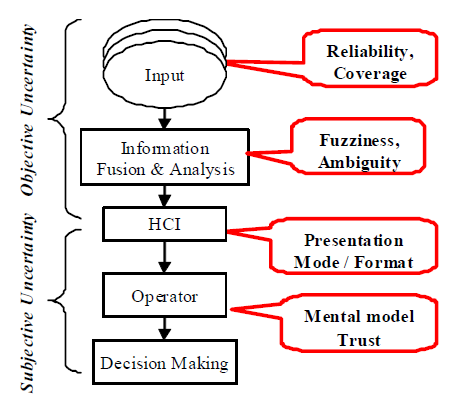
\includegraphics[width=0.7\linewidth,natwidth=898,natheight=587]{billeder/TypesOfUncertainInformation.png}
\caption{Types of uncertainty from \cite{UncertainInformation}}
\label{fig:typesOfUncertainty}
\end{figure}  
The objective uncertainties is the acquisition and processing of the data, and the output. Is the data acquired from a trusted source, is it comprehensive enough and does processing impact the data precision. We are combining and comparing information from different sources during the data processing which can bring uncertainties such as conflicting data or just bad estimates. This information needs to be brought to the users attention so they can act on it. The subjective uncertainties arise in the mind of the user when he is to make a decision. People perceive, interpret and process information differently depending on their background. It is not enough to simply present the information. It is essential to visualize and present the information specifically to the users of the system. Decisions also depend on the specific task, the context, needed accuracy, time constraint, level of risk and experience. 
\\[0.5cm]
Five strategies for user decision making in an uncertain environment is presented in \cite{UncertainInformation}. 
\begin{itemize}
\item Reduction: collecting further information to reduce uncertainty.
\item Assumption-based reasoning: Fill in gaps by relying on experience and imagination, or make sense of factual information.
\item Weighting pros and cons of alternatives
\item Forestalling: Prepare what to do in case of a potential negative result
\item Suppressing uncertainty by simply ignoring it. Last resort.
\end{itemize}  
This emphasizes the need for making the users aware of potential uncertainties in the information e.g. situation awareness. What strategy to use relies greatly on how much uncertainty. The uncertainties should always be made aware to the users so that it is not necessary for them to check the validity themselves. It is furthermore important that the user understands the basic logic of the algorithm so that the answer is not just "black magic". They need to trust it.
\\[0.5cm]
The way of presenting information greatly impacts the decision making process. People can process more data and do it more quickly when it is presented graphically rather than in text \cite{UncertainInformation}. This does not imply that the information can be overloaded with graphical information; it is still important to only show what is most critical for the user to make the best decision. An example of a graphical representation that is perceived quickly is \textit{blurred or degraded graphical images} where the images in a natural way visualizes the amount of uncertainty by blurring it accordingly (see figure ~\ref{fig:blurryIcons}). 
\begin{figure}[h!]
\centering
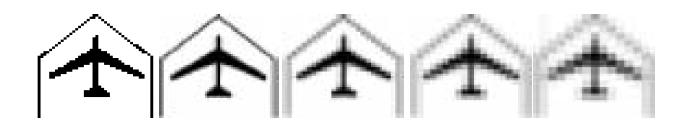
\includegraphics[width=0.7\linewidth,natwidth=898,natheight=587]{billeder/blurryIcons.png}
\caption{Blurry icons from \cite{UncertainInformation}}
\label{fig:blurryIcons}
\end{figure}  
\\[0.5cm]
Based on the discussions in \cite{UncertainInformation} they present a number of high level guidelines for presenting uncertainty. To summarise the most prominent:
\begin{itemize}
\item Always define and present uncertainty and accuracy of data.
\item Present uncertainty at all time and not only when the decision has to be made.
\item Identify the user so that the system can be aligned with their way of reasoning and thinking. This include basic understanding of the underlying algorithm.
\item Provide conflict in data if it is present.
\item Graphical distortion can be improve performance when showing uncertainties.
\item Graphical presentation is not as precise a numerical but they can support each other in achieving precision and performance.
\item Users must be able to restructure the information environment themselves so that it fits their need and way of thinking.
\end{itemize}
The guidelines can be used when developing interface prototypes for Decision Support Systems (DSS).
\subsection{Summary}
KRIST SKRIVER OM DSS.

Decision Support System interfaces must integrate and show uncertain information. The users must be made aware of any information that can have an affect on their decision. Guidelines for visualizing and structuring of information to support the best decision making is presented. These can be used as a starting point for our DSS.

%%%%%%%%%%%%%%%%%%%%%%%%%%%%%%%%%%%%%%%%%%%%%%%%%%%%%%%%%%%%%%%%%%%%%%%

\chapter{Conclusion}
\label{ch:conclusion}

\todo{\dots}

%%%%%%%%%%%%%%%%%%%%%%%%%%%%%%%%%%%%%%%%%%%%%%%%%%%%%%%%%%%%%%%%%%%%%%%


\addcontentsline{toc}{chapter}{Bibliography}
\bibliographystyle{plain} 
\bibliography{refs}

\end{document}

